\chapter{Experimental Evaluation}\label{ch:experimental_evaluation}

This chapter presents results of experiments that were conducted in order to evaluate the use of DRL for robotic grasping with 3D octree-based observations. The created simulation environment is analysed with respect to the feasibility of sim-to-real transfer in order to validate the applicability of all results for use in real-world domain. Furthermore, various configurations and ablations are studied to provide comparative investigation of different approaches and their advantages for learning robotic manipulation with DRL.


\section{Experimental Setup}

All experiments utilise simulation environment for the training of all RL agents. Generalisation to novel objects is evaluated for all agents in the same simulation but on a testing dataset, where one of the trained agents is in addition evaluated also on a real robot to investigate sim-to-real capabilities.


\subsection{Simulation}

Unless otherwise stated, the training in simulation is identical to the setup described in \autoref{sec:impl_simulation_environment} with full-scale domain randomisation. UR5 robot with RG2 gripper is utilised as the primary robot for all experiments because it is the robot that is also tested in real-world domain. However,  Panda robot is also used to train one of the agents. Panda is in addition used to evaluate possible generalisation to new robots with a transfer of an agent trained on UR5, and vice versa. The same random seed is used to train all agents.

When evaluating the trained agents, testing datasets for both object models and PBR textures are used. The environment is configured to present the agent with the full task, i.e.~the largest possible workspace and maximum number of objects. Each episode can last at most~100 time steps and agent succeeds only if an object is lifted~12.5~cm above the ground. The random seed is changed for all evaluated agents to a new common value that is different from a seed used during training. In order to encourage reproducibility, this simulation setup is available as a pre-built Docker image\footnote{\href{https://hub.docker.com/r/andrejorsula/drl_grasping}{https://hub.docker.com/r/andrejorsula/drl\_grasping}}.


\subsection{Real}\label{subsec:real_setup}

Real world setup shown in \autoref{fig:real_setup} is used to evaluate sim-to-real transfer. This setup consists of a UR5 robot with RG2 gripper and Intel RealSense D435\footnote{\href{https://intelrealsense.com/depth-camera-d435}{https://intelrealsense.com/depth-camera-d435}} RGB-D camera that is mounted on a tripod in front of the robot. Pose of the camera with respect to the robot is calibrated with a procedure described in \hyperref[app:camera_pose_calibration]{appendix~\ref*{app:camera_pose_calibration}}. Similarly, \hyperref[app:camera_configuration_and_postprocessing]{appendix~\ref*{app:camera_configuration_and_postprocessing}} presents configuration of the camera and post-processing of its output.

\begin{figure}[ht]
    \centering
    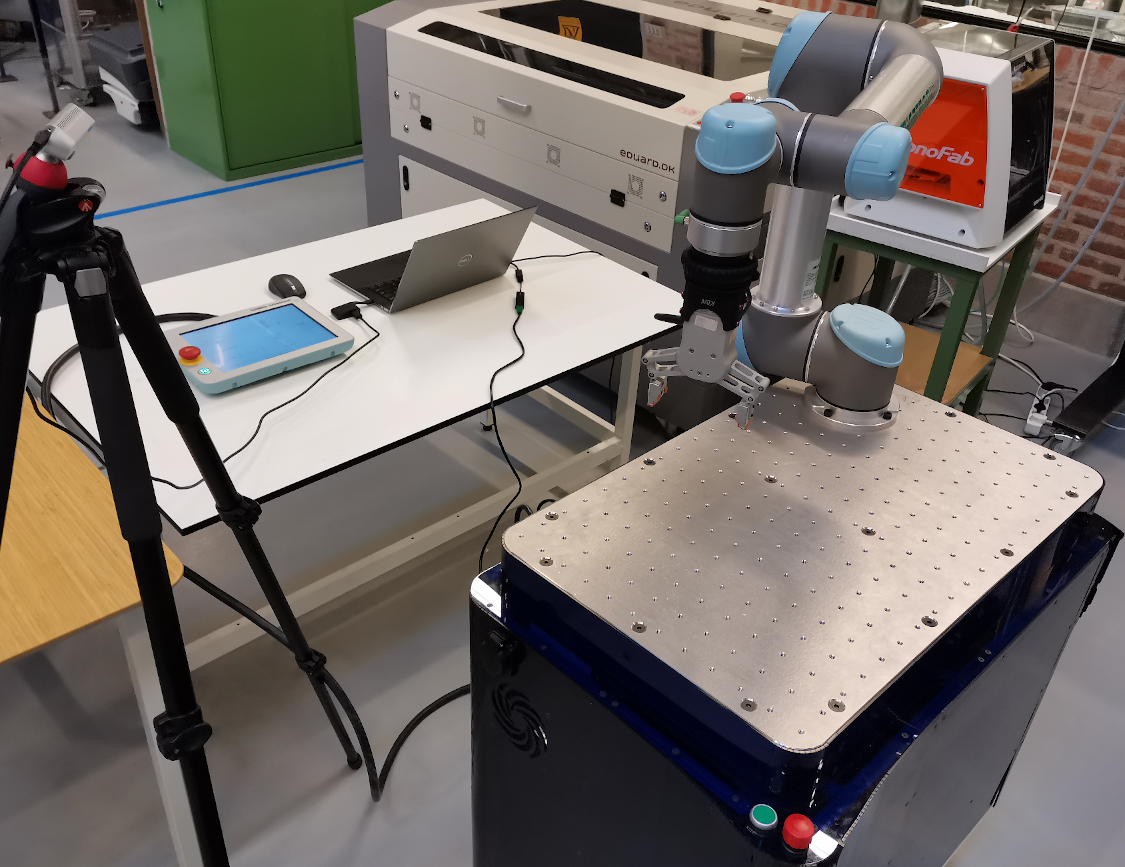
\includegraphics[width=0.66\textwidth]{experimental_evaluation/real_setup.png}
    \caption{UR5 robot with RG2 gripper and RealSense D435 camera in a setup that is used to evaluate sim-to-real transfer.}
    \label{fig:real_setup}
\end{figure}

\autoref{fig:real_objects} shows~18 different objects that were used in real world during the testing. Mostly compliant objects were selected in order to reduce the risk of damage to the gripper due to the unpredictability of end-to-end RL policy trained in a different domain. The same workspace volume and number of objects are used as in the simulation. Similarly, the goal of the agent is to lift an object within~100 time steps.

\begin{figure}[ht]
    \centering
    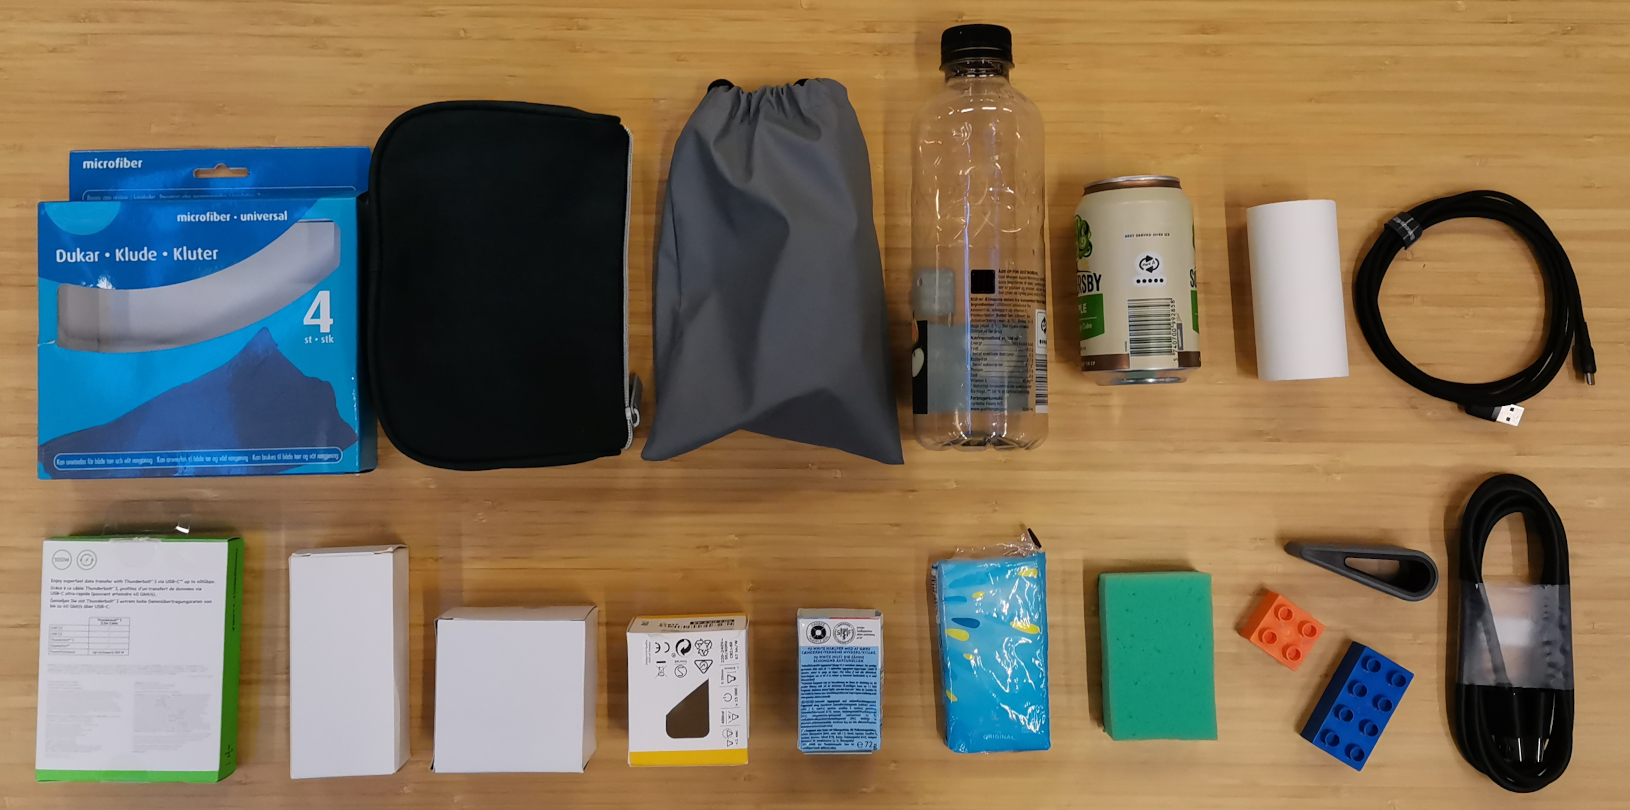
\includegraphics[width=0.66\textwidth]{experimental_evaluation/real_objects.png}
    \caption{A set of 18 objects that were used during the evaluation of sim-to-real transfer.}
    \label{fig:real_objects}
\end{figure}


\section{Results}

Results of the following experiments are presented in this section. First, actor-critic algorithms are compared on the created simulation environment in order to select the best performing one for the task of robotic grasping. Hereafter, octree-based 3D observations are compared to traditional 2D and 2.5D image observations, and studied with respect to camera pose invariance. Similarly, invariance to the utilised robot is evaluated for both training process and transfer of already learned policy. Lastly, results of sim-to-real transfer are presented.

All agents were trained over the duration of~500,000 time steps, which is assumed to provide a comparative analysis among the different experiments from this work. It is expected, that the final performance for many of these agents can be improved with a longer training duration. On average, each agent takes~65~hours to complete~500,000 steps while training on a laptop with Intel Core i7-10875H CPU and Nvidia Quadro T2000 GPU. Therefore, only a single random seed is employed for all agents due to the time-consuming training procedure and time constraints. However, use of several different seeds with a longer training duration is encouraged as it would provide more definitive results. During the training of each agent, success rate is logged for grasps on the training dataset while the agent follows its current stochastic policy that contains exploration noise. After training, each agent is evaluated on novel scenes for~200 episodes, where deterministic actions are selected each step based on the learned policy.

\subsection{Comparison of Actor-Critic Algorithms}

TQC, SAC and TD3 were trained using the same grasping environment with a network architecture presented in \autoref{subsec:actor_critic_network_architecture} and hyperparameters from \hyperref[app:hyperparameters]{appendix~\ref*{app:hyperparameters}}. The success rate during training and the final success rate on novel objects and textures is presented in \hyperref[fig:training_curve_comparison_actor_critic_algorithms]{\figurename~\ref*{fig:training_curve_comparison_actor_critic_algorithms}~\&~\tablename~\ref*{tab:training_curve_comparison_actor_critic_algorithms}} for all three algorithms. The episode lengths of successful episodes are also logged in order to determine how fast an agent can grasp previously unseen objects.

\begin{figure}[ht]
    \centering
    \begin{subfigure}[ht]{0.5845\textwidth}
        \centering
        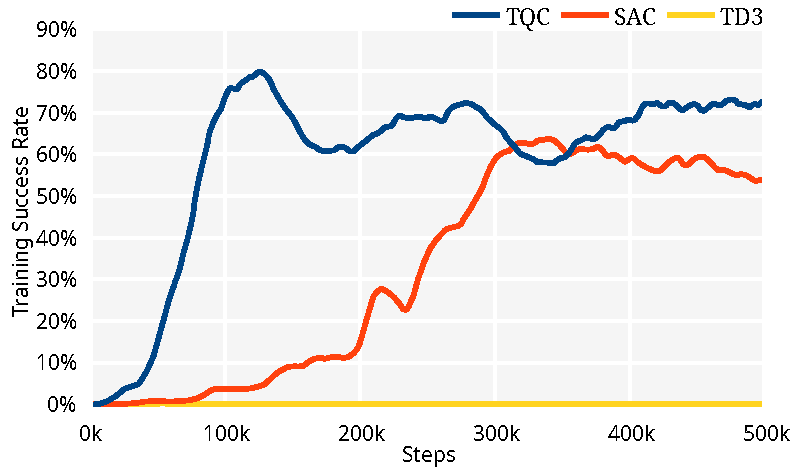
\includegraphics[width=1.0\textwidth]{experimental_evaluation/results_actor_critic.pdf}
    \end{subfigure}%
    ~%
    \begin{subfigure}[ht]{0.4115\textwidth}
        \centering
        \begin{tabular}{c|ccc}
                                          & \textbf{TQC} & \textbf{SAC} & \textbf{TD3} \\ \hline
            \begin{tabular}[c|]{@{}c@{}}Success\\Rate\end{tabular} & 77\%         & 64\%         & 0\%          \\[4mm]
            \begin{tabular}[c|]{@{}c@{}}Episode\\Length\end{tabular} & 14.0         & 29.8         & ---
        \end{tabular}
        \caption*{\textit{Evaluation on novel scenes}}
    \end{subfigure}%
    \captionsetup{labelformat=figure_and_table}
    \addtocounter{figure}{-1}
    \addtocounter{table}{1}
    \captionlistentry[table]{}
    \label{tab:training_curve_comparison_actor_critic_algorithms}
    \caption{Comparison of TQC, SAC and TD3 algorithms on the created grasping environment. The training success rate is processed with a moving average,~\(n = 100\), and exponential smoothing,~\(\alpha = 0.002\), for all agents.}
    \label{fig:training_curve_comparison_actor_critic_algorithms}
\end{figure}

Based on these results, TQC is utilised for all subsequent experiments.


\subsection{Comparison of 2D/2.5D/3D Observations}\label{subsec:comparison_of_2d_2_5d_3d_observations}

3D octree observations are now compared to more traditional 2D RGB and 2.5D RGB-D observations. Besides the success rate, this comparison also includes computational complexity in terms of memory usage and processing time. For octrees, feature extractor from \autoref{subsec:feature_extraction} is used. For RGB and RGB-D images, an analogous CNN feature extractor described in \hyperref[app:feature_extraction_from_rgb_and_rgbd_observations]{appendix~\ref*{app:feature_extraction_from_rgb_and_rgbd_observations}} is employed instead.  In order to make the comparison fair, the same architecture design is used with approximately the same number of learnable parameters as listed in \autoref{tab:feature_extractor_number_of_learnable_parameters_comparison}. TQC hyperparameters from \hyperref[app:hyperparameters]{appendix~\ref*{app:hyperparameters}} are used for all agents. In order to utilise the same replay buffer size for all three agents, the resolution of RGB images and depth maps had to be reduced to~128\({\times}\)128~px for all observation types, including octrees. Note that the change of image resolution does not impact the number of learnable parameters for octrees.

\begin{table}[ht]
    \centering
    \begin{tabular}{l|ccc}
                             &
        \textbf{Octree}      & \textbf{RGB-D} & \textbf{RGB}           \\ \hline
        Learnable Parameters & 226,494        & 229,680      & 229,248
    \end{tabular}
    \caption{Number of learnable parameters per each observation stack for the utilised octree-based, RGB and RGB-D feature extractors.}
    \label{tab:feature_extractor_number_of_learnable_parameters_comparison}
\end{table}

The three different feature extractors are first trained in the fully randomised environment. However, as results in \hyperref[fig:training_curve_comparison_2d_2_5d_3d_random_camera_pose]{\figurename~\ref*{fig:training_curve_comparison_2d_2_5d_3d_random_camera_pose}~\&~\tablename~\ref*{tab:training_curve_comparison_2d_2_5d_3d_random_camera_pose}} indicate, 2D and 2.5D observations are unable to provide invariance to camera pose.

\begin{figure}[ht]
    \centering
    \begin{subfigure}[ht]{0.5845\textwidth}
        \centering
        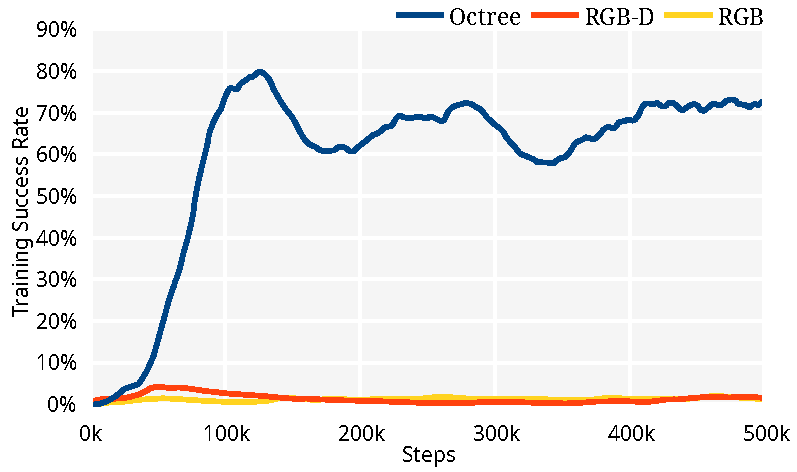
\includegraphics[width=1.0\textwidth]{experimental_evaluation/results_2d_25d_3d_random_camera_pose.pdf}
    \end{subfigure}%
    ~%
    \begin{subfigure}[ht]{0.4115\textwidth}
        \centering
        \begin{tabular}{c|ccc}
                                          & \textbf{Octree} & \textbf{RGB-D} & \textbf{RGB} \\ \hline
            \begin{tabular}[c|]{@{}c@{}}Success\\Rate\end{tabular} & 77\%            & 5\%            & 3\%          \\[4mm]
            \begin{tabular}[c|]{@{}c@{}}Episode\\Length\end{tabular} & 14.0            & 36.5           & 51.0
        \end{tabular}
        \caption*{\textit{Evaluation on novel scenes}}
    \end{subfigure}%
    \captionsetup{labelformat=figure_and_table}
    \addtocounter{figure}{-1}
    \addtocounter{table}{1}
    \captionlistentry[table]{}
    \label{tab:training_curve_comparison_2d_2_5d_3d_random_camera_pose}
    \caption{Results of octree-based, RGB and RGB-D feature extractors on the full environment that randomises camera pose on each episode.}
    \label{fig:training_curve_comparison_2d_2_5d_3d_random_camera_pose}
\end{figure}

Therefore, this experiment is repeated for an environment where the camera pose is static and remains unchanged throughout the entire training and subsequent evaluation on novel scenes. \hyperref[fig:training_curve_comparison_2d_2_5d_3d_fixed_camera_pose]{\figurename~\ref*{fig:training_curve_comparison_2d_2_5d_3d_fixed_camera_pose}~\&~\tablename~\ref*{tab:training_curve_comparison_2d_2_5d_3d_fixed_camera_pose}} provide results for such environment with reduced domain randomisation.

\begin{figure}[ht]
    \centering
    \begin{subfigure}[ht]{0.5845\textwidth}
        \centering
        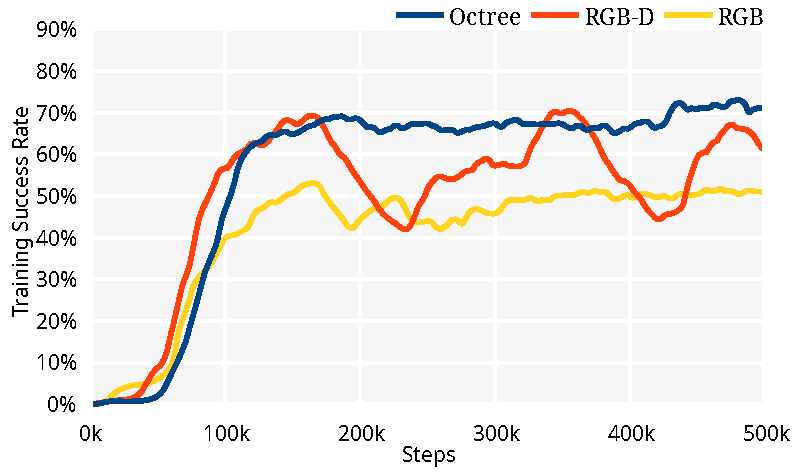
\includegraphics[width=1.0\textwidth]{experimental_evaluation/results_2d_25d_3d_static_camera_pose.pdf}
    \end{subfigure}%
    ~%
    \begin{subfigure}[ht]{0.4115\textwidth}
        \centering
        \begin{tabular}{c|ccc}
                                           & \textbf{Octree} & \textbf{RGB-D} & \textbf{RGB} \\ \hline
            \begin{tabular}[c|]{@{}c@{}}Success\\Rate\end{tabular} & 81.5\%          & 59\%           & 35\%         \\[4mm]
            \begin{tabular}[c|]{@{}c@{}}Episode\\Length\end{tabular} & 24.6            & 9.4            & 9.3
        \end{tabular}
        \caption*{\textit{Evaluation on novel scenes}}
    \end{subfigure}%
    \captionsetup{labelformat=figure_and_table}
    \addtocounter{figure}{-1}
    \addtocounter{table}{1}
    \captionlistentry[table]{}
    \label{tab:training_curve_comparison_2d_2_5d_3d_fixed_camera_pose}
    \caption{Results of octree-based, RGB and RGB-D feature extractors on environment with a fixed camera pose.}
    \label{fig:training_curve_comparison_2d_2_5d_3d_fixed_camera_pose}
\end{figure}

\newpage

Lastly, a comparison of memory usage and computational time for the three observation types and feature extractors is presented in \autoref{tab:feature_extractor_memory_and_computational_time}.

\begin{table}[ht]
    \centering
    \begin{tabular}{r|ccc}
                                                        &
        \textbf{Octree}                                 & \textbf{RGB-D}             & \textbf{RGB}                                     \\ \hline
        Shape \textit{(per sample)}                     & 16\(\times\)16\(\times\)16 & 128\(\times\)128       & 128\(\times\)128        \\
        Cell Count \textit{(per sample)}                & 4,096 octets (theoretical) & 16,384 px              & 16,384 px               \\
        \multirow{2}{*}{Size \textit{(per sample)}}     & 27 kB (average)            & \multirow{2}{*}{49 kB} & \multirow{2}{*}{115 kB} \\
                                                        & 44 kB (maximum)            &                        &                         \\ \hline
        Pre-processing \textit{(average, per sample)}   & 7.2 ms                     & ---                    & ---                     \\
        Batch Formation \textit{(average, batch of 32)} & 3.2 ms                     & 19.7 ms                & 11.2 ms                 \\
        Forward \textit{(average, batch of 32)}         & 2.1 ms                     & 0.8 ms                 & 0.7 ms                  \\
        TQC Update \textit{(average, batch of 32)}      & 32.4 ms                    & 141.7 ms               & 82.3 ms
    \end{tabular}
    \caption{Comparison of computational complexity for octree-based, RGB and RGB-D observations with their corresponding feature extractors. Pre-processing of octrees is performed during data collection and consists of point cloud processing, estimation of normals and creation of octree. Colour features are stored in octree as 32-bit floating point values, whereas RGB and RGB-D utilise byte arrays for memory efficiency in order to allow use of the same replay buffer size. Therefore, the time of batch formation includes conversion of colour channels to floating point values for RGB and RGB-D images.}
    \label{tab:feature_extractor_memory_and_computational_time}
\end{table}

\newpage

\subsection{Invariance to Robot}

In addition to training agents with octree observations on UR5 robot with RG2 gripper, an agent is also trained on Panda robot in order to study the robustness of state-of-the-art actor-critic algorithm with octree observations to different kinematic chains and gripper designs. Comparison of success rate between UR5 and Panda can be seen in \hyperref[fig:invariance_to_robot]{\figurename~\ref*{fig:invariance_to_robot}~\&~\tablename~\ref*{tab:invariance_to_robot}}.

\begin{figure}[ht]
    \centering
    \begin{subfigure}[ht]{0.5845\textwidth}
        \centering
        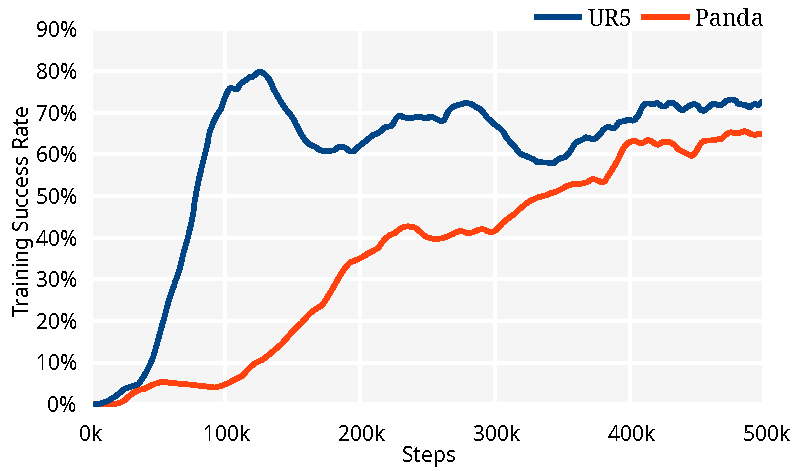
\includegraphics[width=1.0\textwidth]{experimental_evaluation/results_ue5_panda_robot.pdf}
    \end{subfigure}%
    ~%
    \begin{subfigure}[ht]{0.4115\textwidth}
        \centering
        \begin{tabular}{c|cc}
                                           & \textbf{UR5} & \textbf{Panda} \\ \hline
            \begin{tabular}[c|]{@{}c@{}}Success\\Rate\end{tabular} & 77\%         & 61.5\%         \\[4mm]
            \begin{tabular}[c|]{@{}c@{}}Episode\\Length\end{tabular} & 14.0         & 27.1
        \end{tabular}
        \caption*{\textit{Evaluation on novel scenes}}
    \end{subfigure}%
    \captionsetup{labelformat=figure_and_table}
    \addtocounter{figure}{-1}
    \addtocounter{table}{1}
    \captionlistentry[table]{}
    \label{tab:invariance_to_robot}
    \caption{Results of using the same algorithm and hyperparameters on the created environment with UR5 and Panda robots.}
    \label{fig:invariance_to_robot}
\end{figure}

Furthermore, feasibility of transferring a policy trained on one robot to another is investigated. Such transfer is evaluated on novel scenes with a policy trained on both UR5 and Panda. Results for this experiment can be found in \autoref{tab:results_robot_transfer}.

\begin{table}[ht]
    \centering
    \begin{tabular}{cr|cc}
                                                        &                & \multicolumn{2}{c}{Evaluation}                  \\
                                                        &                & \textbf{UR5}                   & \textbf{Panda} \\ \hline
        \multirow{2}{*}{\begin{tabular}[c]{@{}c@{}}Training\end{tabular}} & \textbf{UR5}   & 77\%                           & 27.5\%         \\
                                                        & \textbf{Panda} & 75\%                           & 61.5\%
    \end{tabular}
    \caption{Comparison of success rate on novel scenes for policies trained on one robot and evaluated on another, for UR5 with RG2 gripper and Panda robot with its default gripper.}
    \label{tab:results_robot_transfer}
\end{table}

\newpage

\subsection{Sim-to-Real Transfer}

Finally, an agent trained inside simulation is evaluated in real-world domain to study the feasibility of sim-to-real transfer for environment with domain randomisation and octree-based observations. Setup described in \autoref{subsec:real_setup} is used, where objects are randomly replaced after each success or after~100 time steps have elapsed. With this setup,~41 out of~60 episodes were successful, which results in a success rate of~68.3\%. \autoref{fig:sim_to_real_success_examples} shows examples of successful grasps, whereas \autoref{fig:sim_to_real_failure_examples} shows failed attempts. Recording of several episodes is available on YouTube\footnote{\href{https://youtube.com/watch?v=btxqzFOgCyQ&list=PLzcIGFRbGF3Qr4XSzAjNwOMPaeDn5J6i1}{https://youtube.com/watch?v=btxqzFOgCyQ}}, which can be used to qualitatively assess the policy and corresponding grasps.

\begin{figure}[ht]
    \centering
    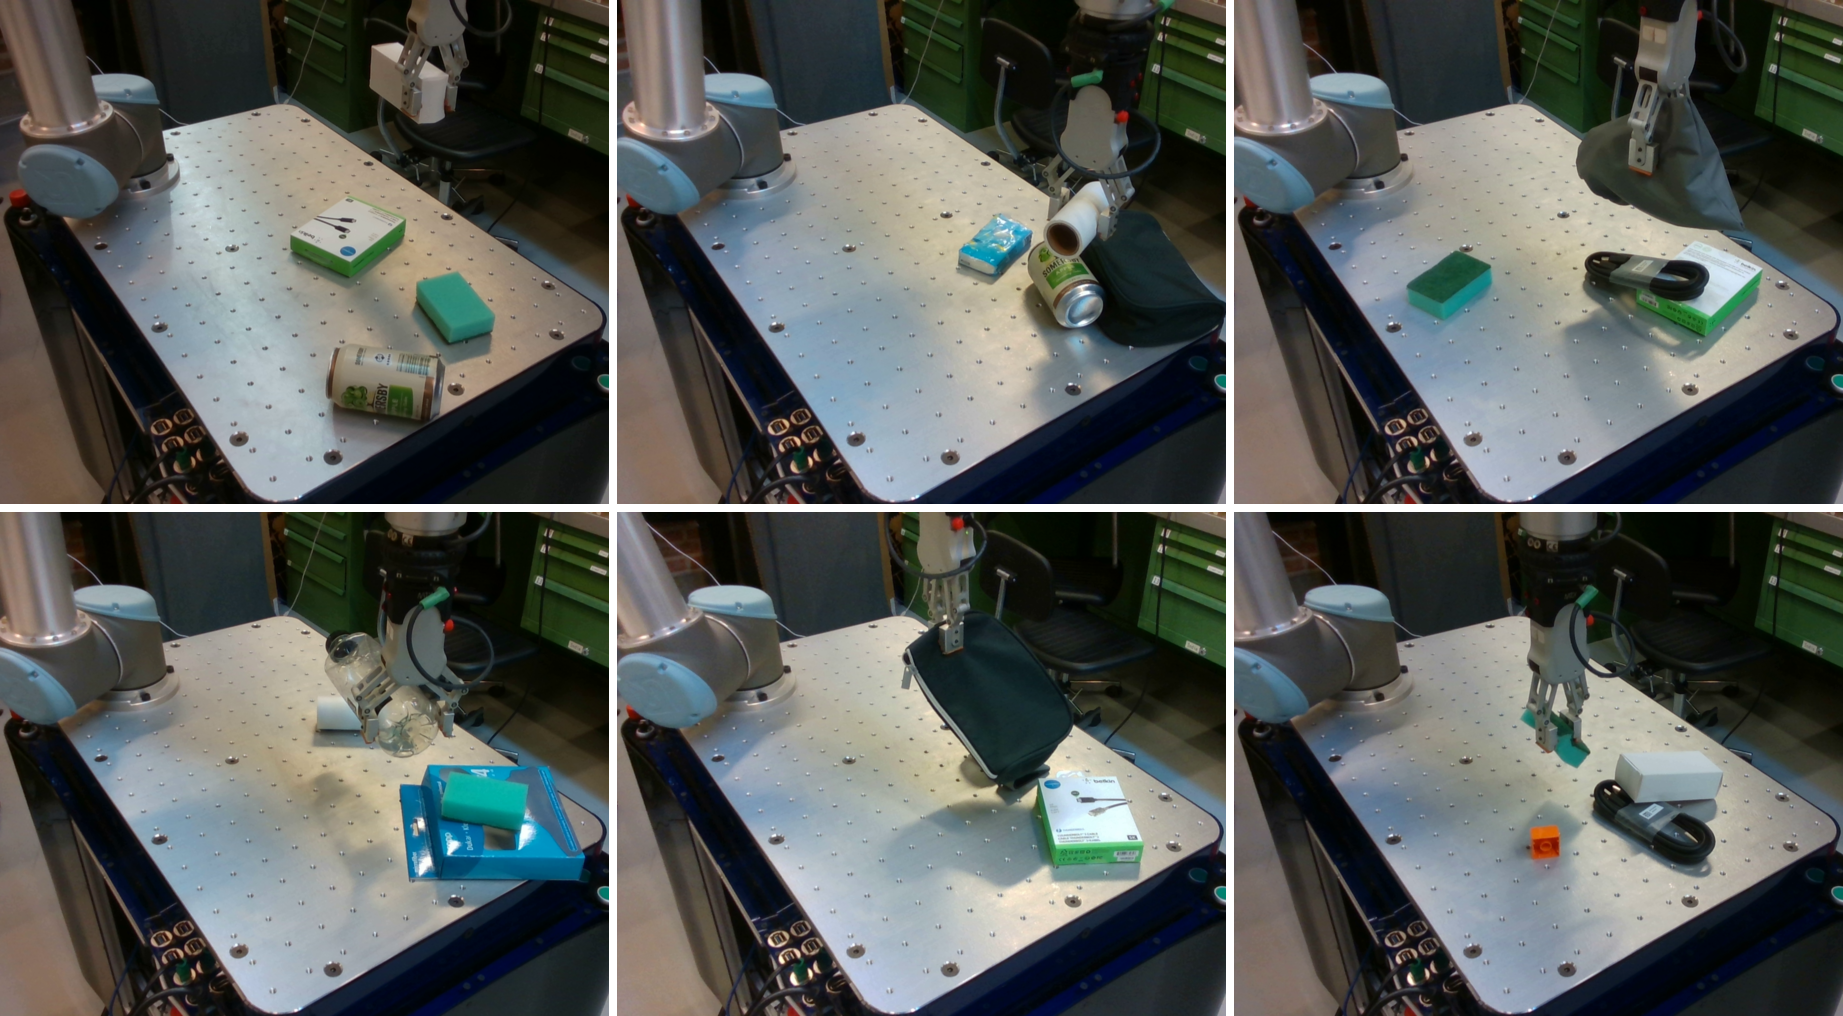
\includegraphics[width=1.0\textwidth]{experimental_evaluation/real_success_examples.png}
    \caption{Examples of successful grasps accomplished by a policy that was transferred from simulation to real-world domain.}
    \label{fig:sim_to_real_success_examples}
\end{figure}

\begin{figure}[ht]
    \centering
    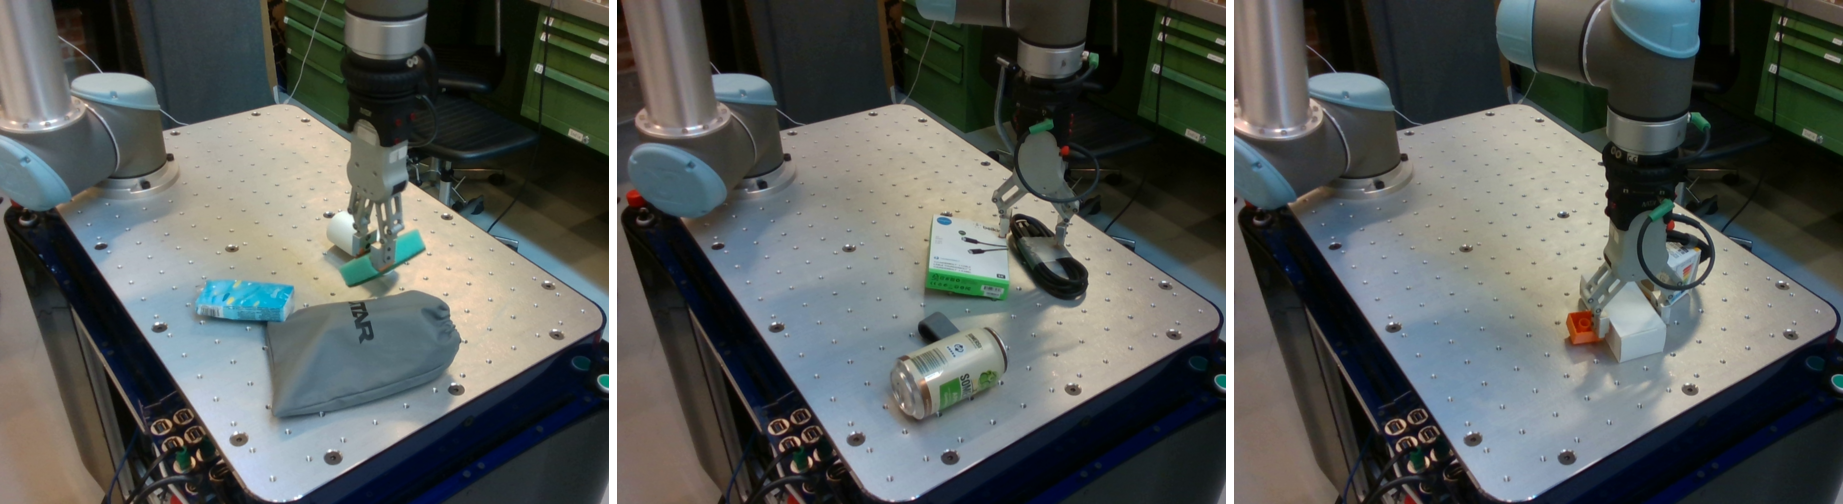
\includegraphics[width=1.0\textwidth]{experimental_evaluation/real_failure_examples.png}
    \caption{Examples of failed attempts. The most common cause of failure is obstruction of a finger by another object, which prevents the RG2 gripper from closing.}
    \label{fig:sim_to_real_failure_examples}
\end{figure}

\newpage

\section{Ablation Studies}

Besides results presented in the previous section, various ablations of the full approach are studied in order to determine their effects and contributions. It is believed that these results are applicable also for other robotics tasks that utilise visual observations. The following ablations and configurations are studied.
\vspace{-\topsep}
\begin{itemize}
    \itemsep -2.5mm
    \item No demonstrations
    \item No curriculum
    \item No colour features
    \item No proprioceptive observations
    \item Separate feature extractors for actor and critics
    \item Shared feature extractor for all stacked observations
\end{itemize}
\vspace{-\topsep}
\hyperref[fig:ablation_studies]{\figurename~\ref*{fig:ablation_studies}~\&~\tablename~\ref*{tab:ablation_studies}} present these ablations with respect to their comparative learning curve and attainable success rate on novel scenes.

\begin{figure}[ht]
    \centering
    \begin{subfigure}[ht]{1.0\textwidth}
        \centering
        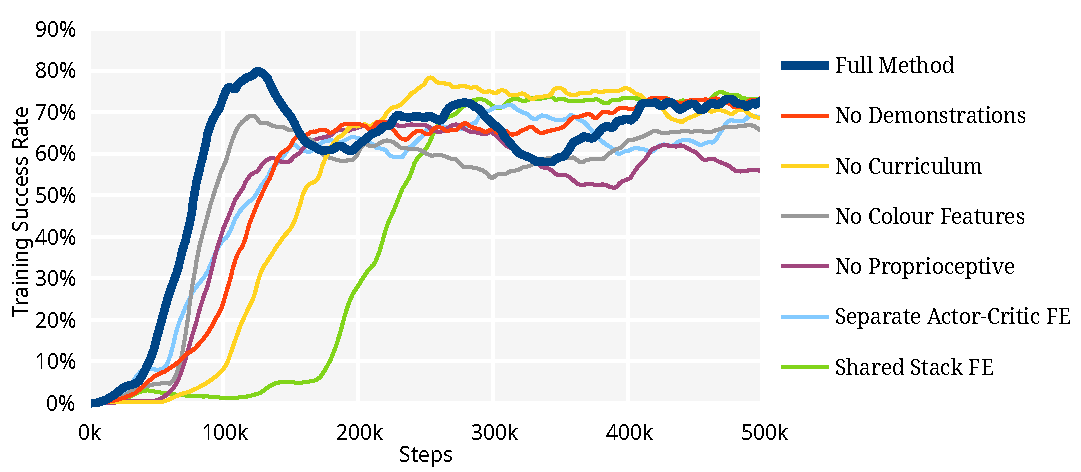
\includegraphics[width=1.0\textwidth]{experimental_evaluation/results_ablation_studies.pdf}
    \end{subfigure}

    \vspace{8mm}

    \begin{subfigure}[ht]{1.0\textwidth}
        \centering
        \begin{tabular}{c|ccccccc}
                                                    &
            \textbf{\begin{tabular}[c]{@{}c@{}}Full\\Method\end{tabular}} &
            \textbf{\begin{tabular}[c]{@{}c@{}}No\\Demon-\\strations\end{tabular}} &
            \textbf{\begin{tabular}[c]{@{}c@{}}No\\Curriculum\end{tabular}} &
            \textbf{\begin{tabular}[c]{@{}c@{}}No\\Colour\\Features\end{tabular}} &
            \textbf{\begin{tabular}[c]{@{}c@{}}No\\Proprio-\\ceptive\end{tabular}} &
            \textbf{\begin{tabular}[c]{@{}c@{}}Separate\\Actor-\\Critic FE\end{tabular}} &
            \textbf{\begin{tabular}[c]{@{}c@{}}Shared\\Stack\\FE\end{tabular}}                                                        \\ \hline
            \begin{tabular}[c|]{@{}c@{}}Success\\Rate\end{tabular}          & 77\% & 84\% & 70.5\% & 66.5\% & 75\% & 68.5\% & 79\% \\[4mm]

            \begin{tabular}[c|]{@{}c@{}}Episode\\Length\end{tabular}          & 14.0 & 24.5 & 19.9   & 29.4   & 23.0 & 27.5   & 22.8
        \end{tabular}
    \end{subfigure}%
    \captionsetup{labelformat=figure_and_table}
    \addtocounter{figure}{-1}
    \addtocounter{table}{1}
    \captionlistentry[table]{}
    \label{tab:ablation_studies}
    \caption{Results of various ablations of the full method. (FE -- Feature Extractor)}
    \label{fig:ablation_studies}
\end{figure}
